\chapter{Progress in Data Abstraction}
\lhead{\emph{Progress in Data Abstraction}}

In this implementation of data abstraction, the aim is to reduce images down to only the boundaries of the objects in the scene and then fill the spaces between theses boundaries with block colours based on the original image. Therefore the general process of the design is:
\begin{enumerate}
    \item Use edge detection on the image, presenting the boundaries of the scene as white lines and the rest as black. 
    \item Divide up the original image into sections that can reasonably be averaged into a single colour, defined by the boundaries produced by the edge detection or otherwise.
    \item Find the average colours (or reasonable alternatives) for these sections.
    \item Flood fill the spaces in the edge detection output with the average colours of the original image.
\end{enumerate}
While this section will be presented in the context of the entire process occurring on a single computer (as this was the testing platform), when incorporated into the final system points 1-3 will be done using the raspberry pi on the rover and point 4 will be done on the computer. This allows for much smaller data packets to be sent over a wireless connection (wifi), due to being able to send the colour information for entire sections of the image as a single colour value.

\section{Edge Detection}

Canny edge detection was implemented using the Canny function provided by OpenCV. The sequence of processes implemented to support the algorithm in producing high quality edges are shown in Figure \ref{fig:CannyProc}. 

\begin{figure}[H]
    \begin{center}
    \begin{tabular}{ c c c }
        (1) & (2) & (3) \\
        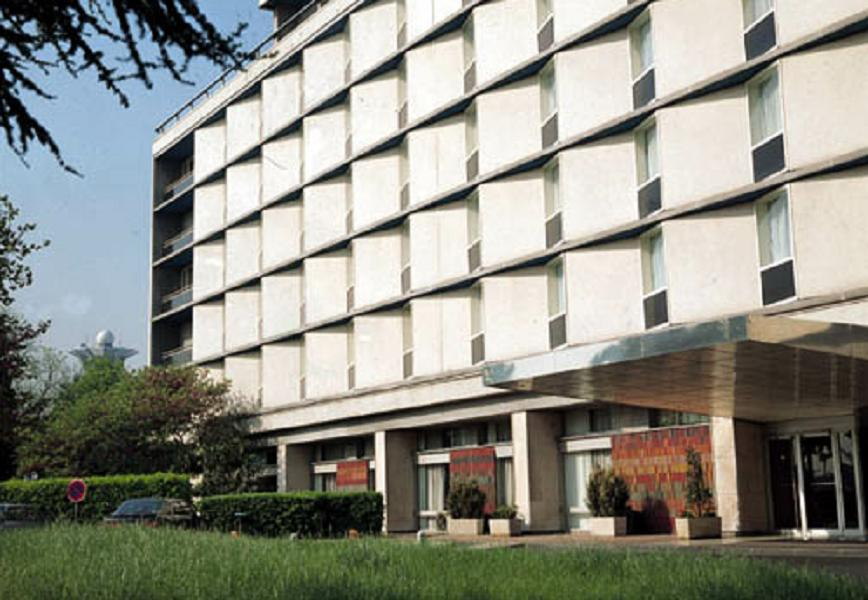
\includegraphics[width=0.31\textwidth]{Figures/building.jpg} &
        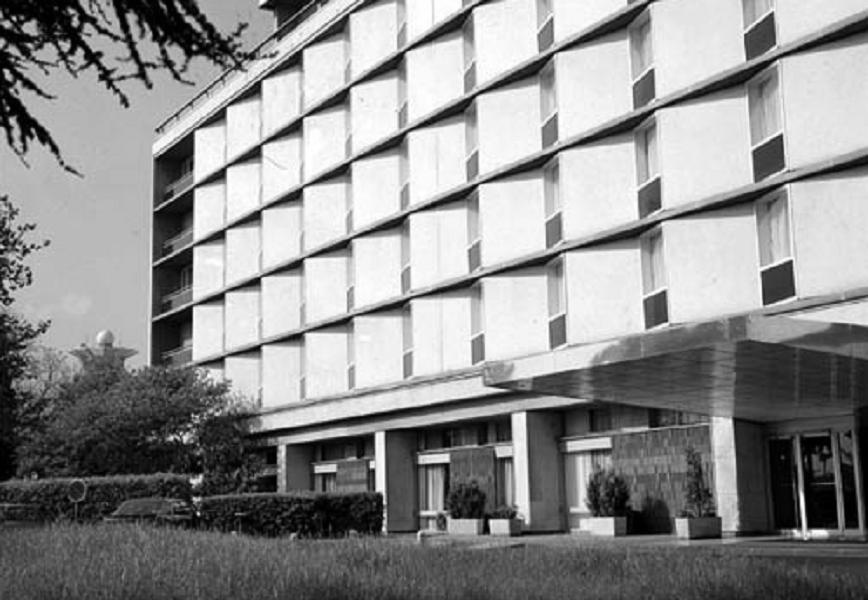
\includegraphics[width=0.31\textwidth]{Figures/buildGray.jpg} &
        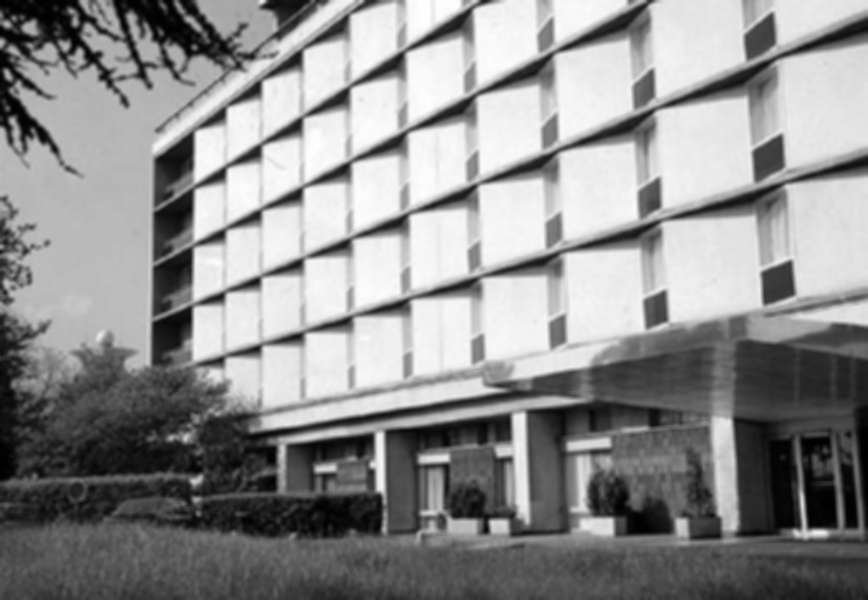
\includegraphics[width=0.31\textwidth]{Figures/buildBlur.jpg}
    \end{tabular}
    \begin{tabular}{ c c }
        (4) & (5) \\
        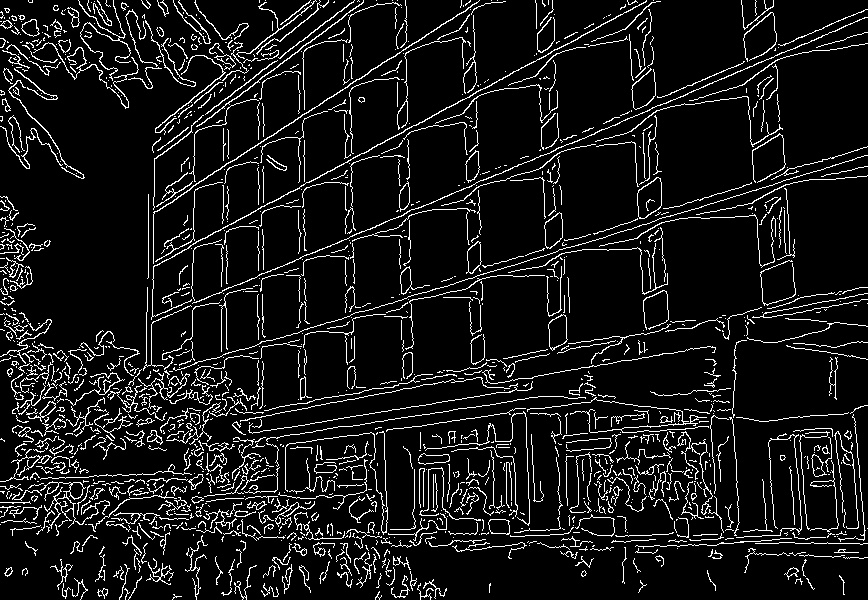
\includegraphics[width=0.31\textwidth]{Figures/buildCanny.jpg} &
        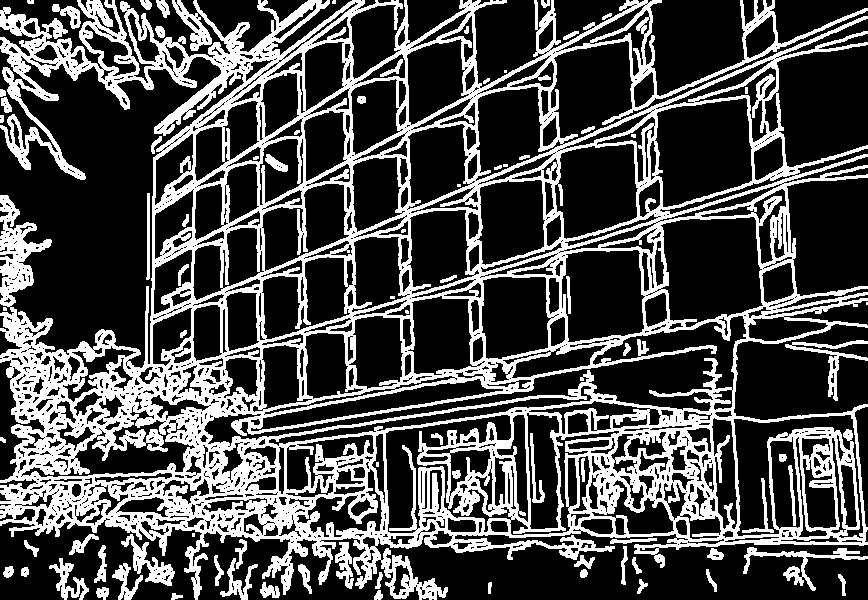
\includegraphics[width=0.31\textwidth]{Figures/buildDilated.jpg}
    \end{tabular}
    \caption[Process of Edge Detection]{(1) the original image, provided by OpenCV, (2) post grayscaling, (3) post blurring, (4) post edge detection, and (5) post dilation.}
    \label{fig:CannyProc}
    \end{center}
\end{figure}

The image is first made grayscale, as Canny detects large changes in light intensity and not colour. The image is then blurred to remove any unnecessary edges and noise that Canny may pick up. The edge detection is used, producing white lines representing the edges on a black background (the details of parameter experimentation with Canny and the previous blurring are presented in Appendix B). The output of the edge detection is finally dilated to make the lines thicker and bridge the gaps between the lines that are very close together. This is done to make the image more cartoon-like and more generally aesthetically pleasing, reduce the number of lines produced by areas that are dense with detail such as hair and foliage (an example of this detail density can be seen in the bush in Figure \ref{fig:Blur}), and to bridge the gaps between lines that are close together, increasing the likelihood of defined shapes being created that can be easily flood filled later.

\section{Flood filling}

Flood filling was chosen as the method for applying colour to the Canny output image, as it is the most efficient way to fill spaces of unknown size and shape that are defined by high contrast boundaries; using it makes dividing up the image into sections unnecessary. To use the OpenCV flood fill function you must provide a seed point to start flooding from, a colour to fill with, and parameters for the filling itself (unchanged from the defaults provided by the OpenCV documentation \cite{opencvffilldemo}).

\subsection{Seed Point}

Finding the points to flood fill from is a challenge, as each image will have a different number of spaces to be filled and the spaces can be anywhere. Three different methods were attempted to solve the problem. The first was an attempt to use OpenCV's contour functionality to provide seed points, however this was unusable due to high resource requirements. The method is detailed in Appendix C.

Although it would by ideal to aim to flood fill from the centre point of each space, it is only necessary if a few specific pixels are being selected to fill from, as each time a line pixel is selected that potential seed point can only be discarded. It is possible to instead iterate through the whole image and flood fill from every pixel found that is not part of a line or an already filled space.

This method is more effective at filling every space than the previous, and is also less resource intensive. However, if presented with a complicated environment with many spaces to flood fill, it must fill every single one, therefore leading to unacceptable drops in frame rate.

The most simple solution to the performance issues caused by allowing the number of times flood fill is used per image to vary would be to set a maximum. However, if this is done the seed points can no longer be selected by iterating through the whole image, as the presence of many small spaces at the top of an image would lead to larger, more important spaces not being filled at the bottom. The solution is to select a set number of points quasi-randomly across the image using Sobol sequencing. Although a certain number of points will land on lines and therefore not be used, if there are enough points then all the important spaces are filled without serious impact on performance. Also, with this method performance is not affected by the complexity of the image, however more complicated images will be processed with many of the more dense areas unfilled (Figure \ref{fig:BrutevsSobol}). For these reasons, the seed points are selected using this method in the current build.

\begin{figure}[H]
    \begin{center}
    \begin{tabular}{ c c }
        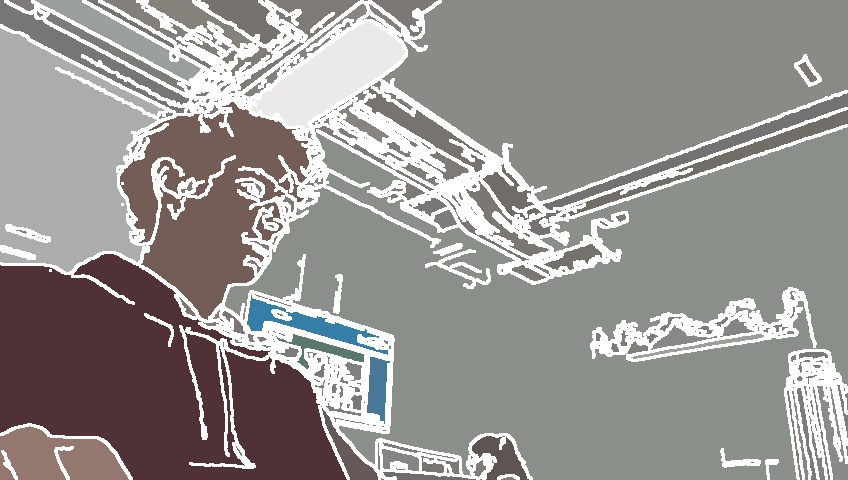
\includegraphics[width=0.45\textwidth]{Figures/Brute.jpg} &
        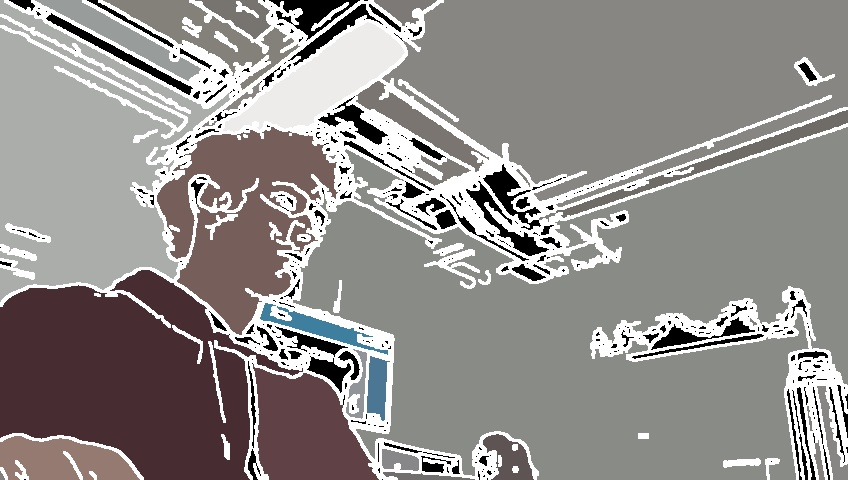
\includegraphics[width=0.45\textwidth]{Figures/Sobol.jpg}
    \end{tabular}
    \caption[Comparison of brute force and Sobol seed point generation]{Comparison of brute force and Sobol seed point generation. It can be clearly seen that the brute force method (left) accurately fills every space in the image, whereas using Sobol results in many unfilled spaces. However, Sobol is higher performance with a frame rate of 17.14fps, compared to 8.57fps using brute force.}
    \label{fig:BrutevsSobol}
    \end{center}
\end{figure}

\subsection{Fill Colour}

Three different methods were considered for finding the colours that the Canny output should be flood filled with. All three methods are valid solutions, but present different ratios between accuracy and resource requirements.

While filling the abstracted image with the average colours present within the input is preferable, it is not essential to the project; provided that the objects in the scene are still recognisable, they don't have to be exactly the right colour. For this reason it would be acceptable to not find the average colour of the area being flood filled at all, and instead simply use the colour of the seed point. This is a very fast method, however produces incredibly inconsistent colours between images. This is because there can be a wide spectrum of colour across a single surface even within the threshold of Canny edge detection, and the Sobol sequence will sample from a different point each time producing spaces that flicker between a wide range of colours.

The consistency of the previous method can be improved substantially with minimal impact on performance by taking an average of the colour within the area of a small circle around the seed point, rather than just the colour of that one point. This significantly improves the consistency between images, however introduces the problem of incorporating pixels from outside the space to be filled. This is due to the quasi-random points often being closer to the edge of the space that they are being flooded from then the radius of the circle. Therefore, the size of the circle must be carefully selected to balance the benefits of increasing size (more consistency when the seed point is further from the edge) and the benefits of decreasing size (more consistency when the seed point is closer to the edge). 

The OpenCV flood fill function provides the ability to fill a blank mask using the boundaries defined by a different image \cite{bradski2008learning}. This makes it possible to create a custom mask with the exact size and shape of the space that is to be filled and use that to find the average colour instead of the predefined circle. This produces the average colour of every space in the image exactly at the expense of adding an extra stage of flood filling before the Canny output itself is filled. The consistency between images for this is the maximum possible based on colour alone (Figure \ref{fig:ColourConsistency}), though inconsistency in the edge detection causes certain spaces to combine and divide constantly, leading to a small amount of colour inconsistency to remain regardless. This method has a noticeable impact on performance, though within acceptable bounds, leading this to be the chosen method for the current build. Examples of the results produced by the final build can be seen in Appendix D.

\begin{figure}[H]
    \begin{center}
      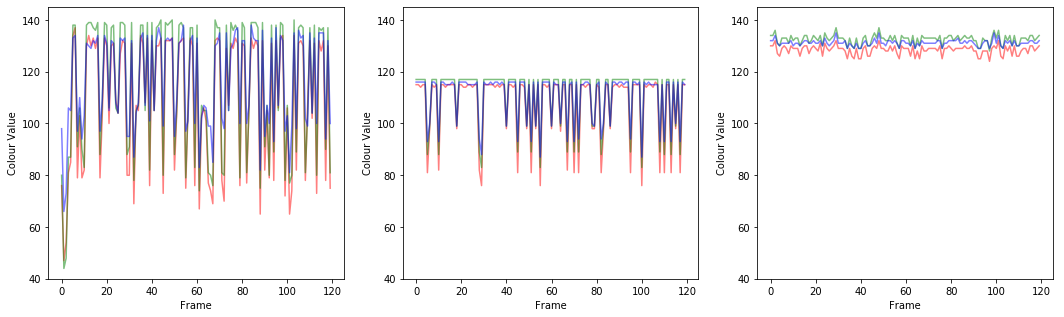
\includegraphics[width=1\textwidth]{Figures/ColourConsistency.png}
      \caption[Comparison of Colour Averaging Methods]{Comparison of Colour Averaging Methods. These are RGB values over time produced by flood filling an example area using the seed point colour (left), circle average (middle), and flood fill average (right). The increase in consistency from left to right is very apparent.}
      \label{fig:ColourConsistency}
    \end{center}
\end{figure}